\chapter{Exposé}

\section{Introduction}

The game 'Who Am I' has various names and exists in numerous forms and variations. Each player can represent virtually anything, which increases the difficulty, and the number of players can also vary. A typical version of the game for children is a $4 \times 6$ board that includes only persons. This version is further referred to for a more specific analysis, but a similar ratio is expected for a scaled-up version.

\section{Theoretical Background and State of the Art}
\label{sec:state-of-the-art}

The field of RL has witnessed significant advancements in recent years, particularly in its application to complex decision-making processes. RL algorithms, inspired by behavioral psychology, have demonstrated remarkable capabilities in learning optimal strategies through trial and error interactions with environments. Concurrently, stochastic modeling techniques have long been employed to analyze uncertainty and randomness in various systems. This includes stochastic processes, which offer powerful frameworks for modeling dynamic systems influenced by probabilistic factors. In the context of the discussed topic, the integration of RL with stochastic approaches presents a promising avenue for addressing challenges such as uncertainty, scalability, and adaptability. Recent research has explored the synergy between RL and stochastic methods in diverse domains, ranging from robotics and game theory to finance and healthcare. By leveraging the strengths of both paradigms, researchers aim to develop more robust and efficient solutions for decision-making tasks in complex and uncertain environments.


\section{Research Question}

These approaches lead to the following research question for this bachelor
thesis:

\begin{quote}
	What is the optimal number of questions required to accurately identify a specific individual out of a set of 24 persons using reinforcement learning and stochastic modeling techniques?
\end{quote}


\section{Methodology}

\iffalse
To answer this question, the bachelor thesis (master thesis) will be realized
as a combination of literature work and practical or prototypical
implementation.

First, the existing literature (extending section \ref{sec:state-of-the-art})
will show how the topic of smooth transition gameplay is dealt with from a
game design perspective. Common factors such as mechanics will be extracted
from this and serve as the basis for a theoretical framework. This framework
will contain a list of core mechanics and guidelines for their application so
that LPD games allow easy entry and a variable number of players.

The applicability of this framework will be tested by an own LPD game developed
during the term project. By asking simple qualitative questions to the players
and observing the visitors during several test runs, it will be determined
whether smooth transition gameplay could be achieved with the mechanics used.
\fi
Discussed in the upcoming exercises...

\section{Expected Results}

The study anticipates two key outcomes: firstly, a detailed analysis of the number of questions required to identify a person from a group of 24 using an RL algorithm. Secondly, a comparative examination of the same scenario employing stochastic modelling techniques. It is expected that the result of both the RL algorithm and the stochastic solution are almost the same.

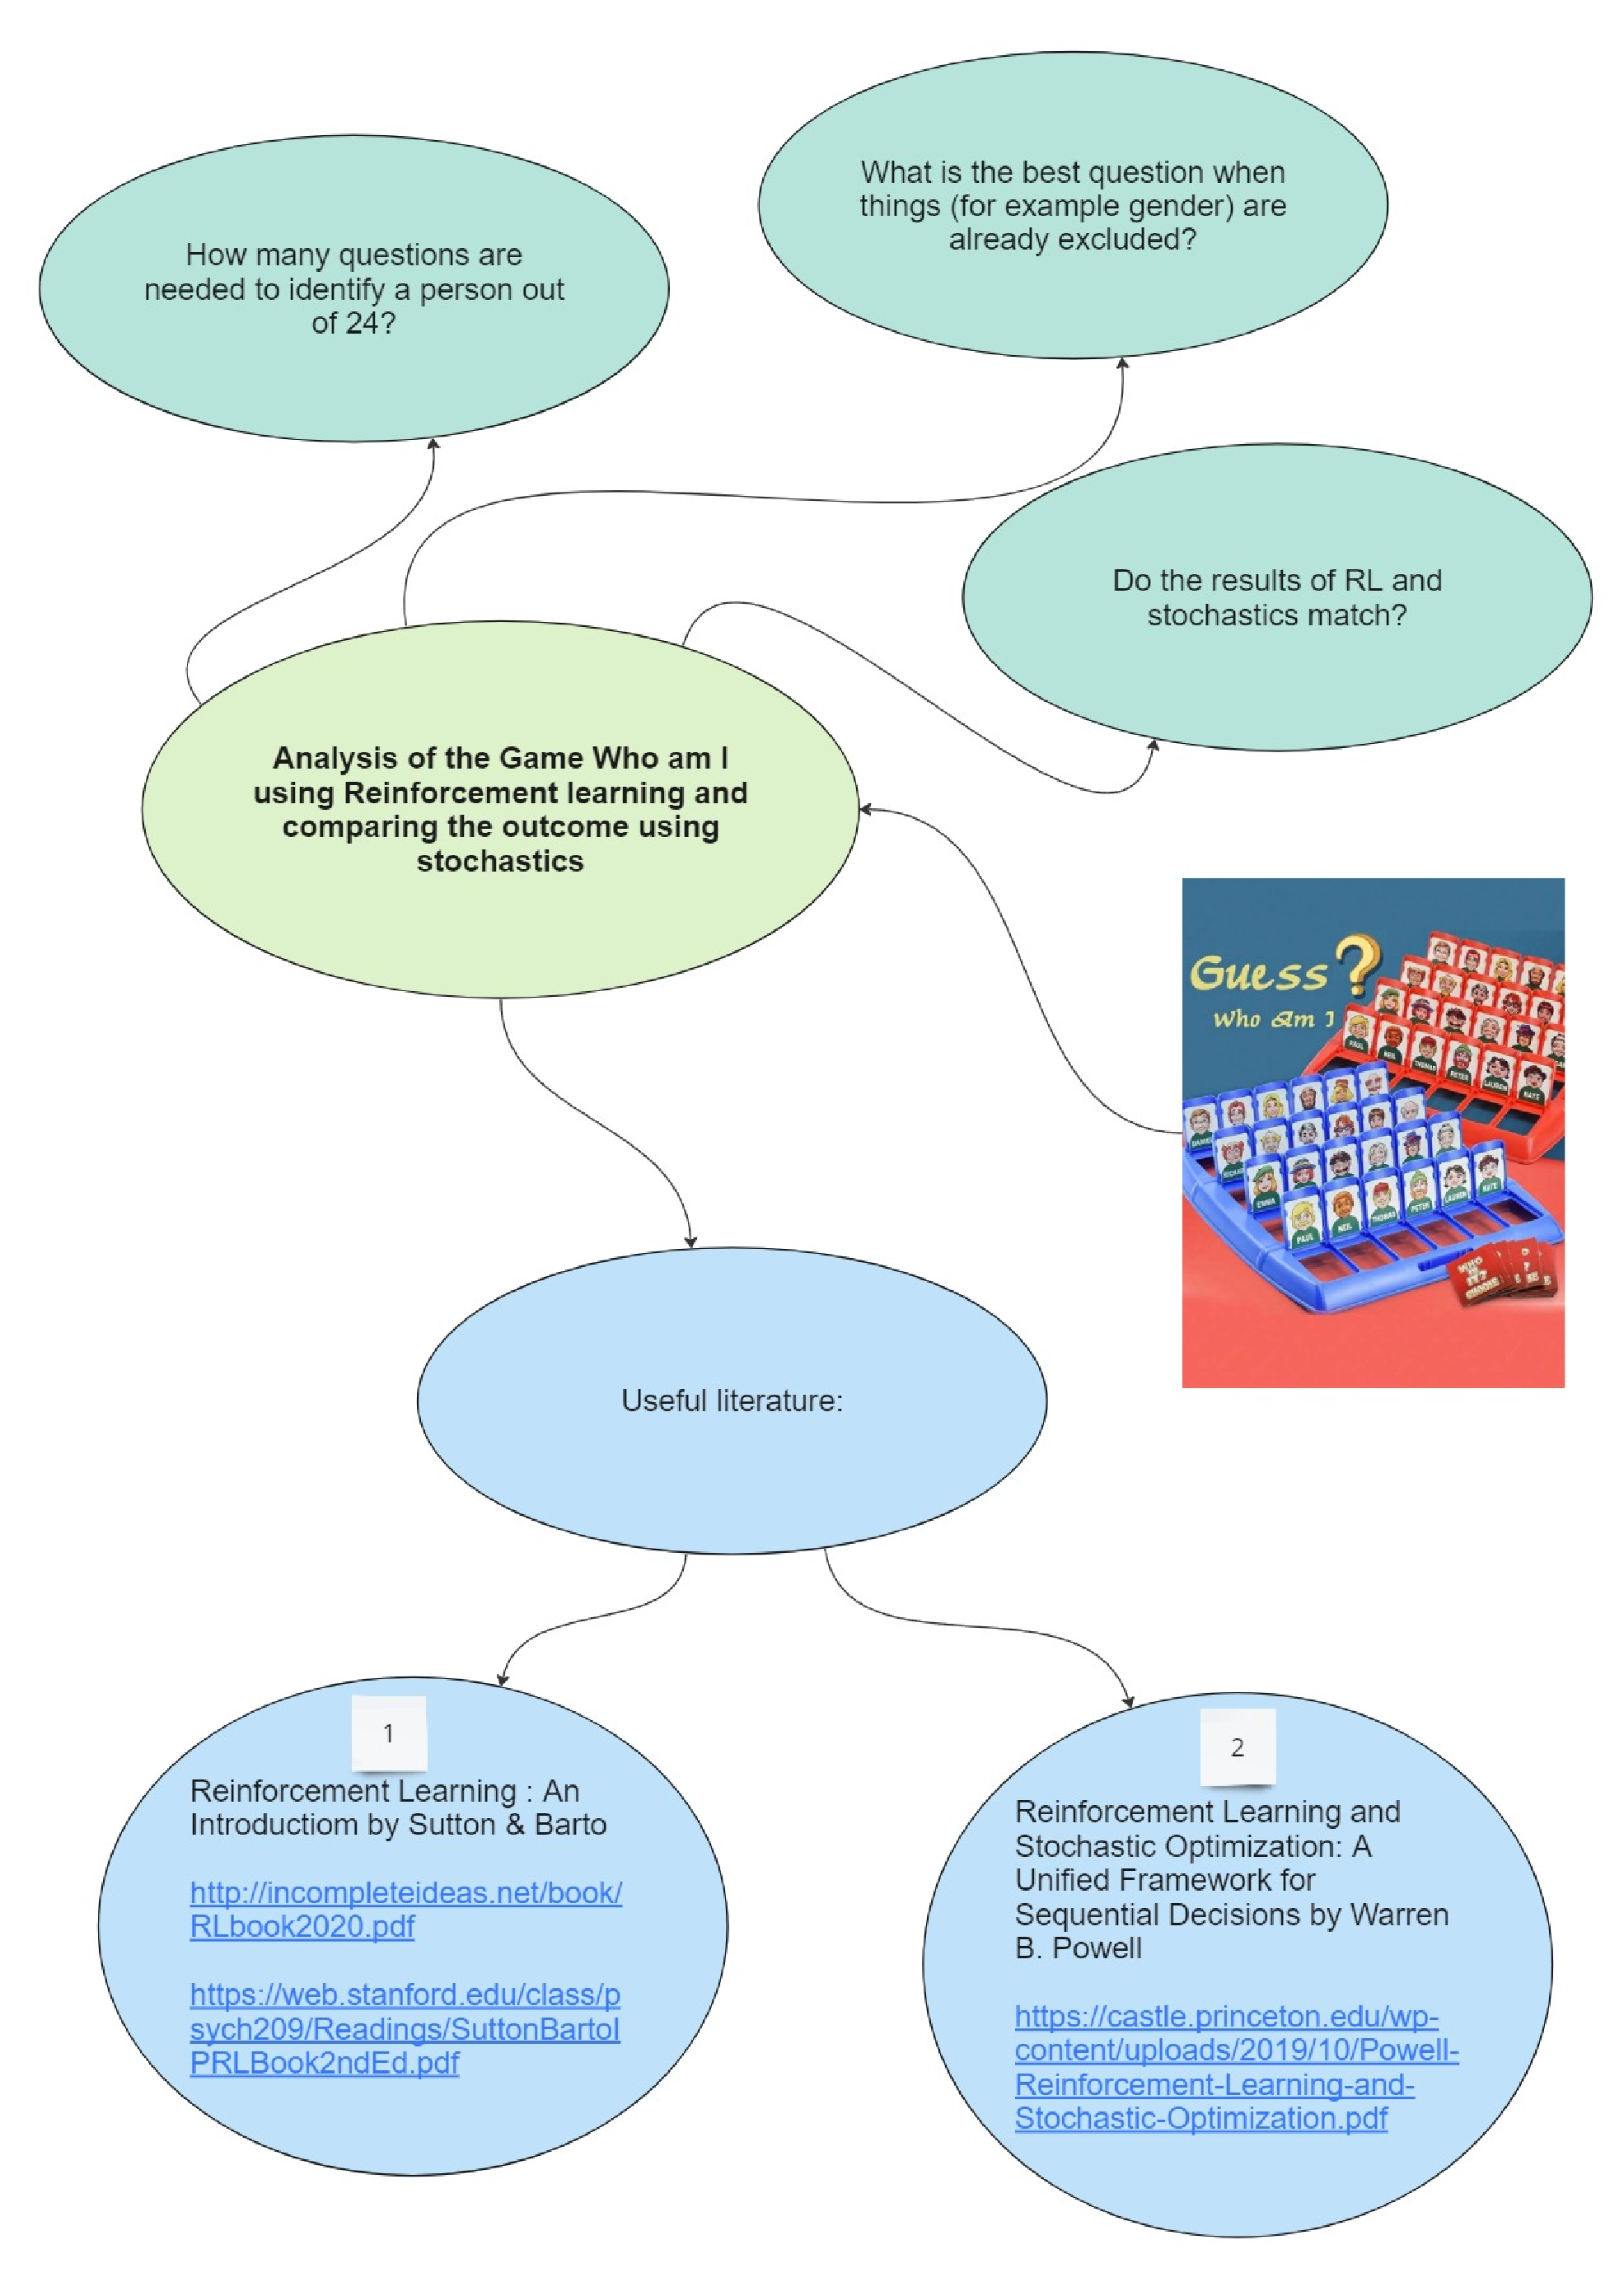
\includegraphics[width=\textwidth]{../pdfs/Mindmap.pdf}